\documentclass[pdftex,british,final,infofoot, biblio,aspectratio=169]{slidedeck}

\usepackage{gla-tikz}
\makeatletter

% larger fonts
\newcommand\HUGE{\@setfontsize\Huge{50}{60}}

% For tikz matrices in beamer
\global\let\tikz@ensure@dollar@catcode=\relax
\makeatother


\title{Type-Theory as a Language Workbench}
\author[Jan de Muijnck-Hughes \and Guillaume Allais \and Edwin Brady]{\underline{Jan de Muijnck-Hughes} \and Guillaume Allais \and Edwin Brady}
\titlegraphic
{%
  
\includegraphics[keepaspectratio,scale=0.8]{gla}
  \hfill
  
\includegraphics[keepaspectratio,scale=1.8]{sta}%
}

\date[EVCS '23]
{%
  Eelco Visser Commemorative Symposium \\ Delft, \origdate\printdate{2023-04-05}%
}

\bibliography{biblio.bib}


\begin{document}

\maketitle

\begin{frame}[fragile]{A Quest: Get on yer bike!}
  \begin{columns}
    \begin{column}{0.2\textwidth}
      \centering
      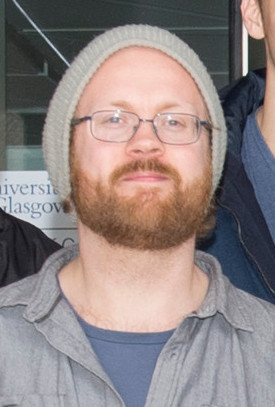
\includegraphics[keepaspectratio,width=0.7\columnwidth]{master}
      \\
      \Huge\noticeBF{Master}
    \end{column}
    \begin{column}{0.5\textwidth}
      \begin{center}
        {\huge\noticeBF{V{\'e}lo}}
      \end{center}
\begin{Verbatim}
   let b = false
in let double
         = (fun x : nat => (add x x))
in let x = (double ?hole)
in         (double ?hole)
\end{Verbatim}

        \begin{block}{}
          The \structure{Simply-Typed Lambda Calculus} with\ldots
          \vspace{-1em}
          \begin{multicols}{2}
            \begin{itemize}
            \item Let-Bindings
            \item Booleans
            \item Natural Numbers
            \item Typed Holes
            \item Elaboration
            \item Optimisations
            \end{itemize}
          \end{multicols}
        \end{block}

    \end{column}
    \begin{column}{0.2\textwidth}
      \centering
      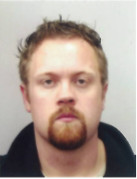
\includegraphics[keepaspectratio,width=0.7\columnwidth]{novice}
      \\
      \Huge\noticeBF{Novice}
    \end{column}
  \end{columns}

\end{frame}

\begin{frame}
  \frametitle{Well\ldots Have you heard of Language Workbenches?}
  \framesubtitle{\url{https://spoofax.dev/}}
  \begin{columns}
    \begin{column}{0.3\textwidth}
      \begin{center}
        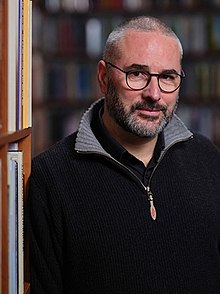
\includegraphics[keepaspectratio,height=0.5\textheight]{visser}
        \\
        \Huge\noticeBF{The Expert}
      \end{center}
    \end{column}
    \begin{column}{0.4\textwidth}
      \begin{tikzpicture}
        \node (c) {
\includegraphics[width=\columnwidth,keepaspectratio]{spoofax}};
        \node (d) [above = of c, OrangeTitle] {Description};
        \node (i) [below = of c, OrangeTitle] {Implementation};

        \foreach \s/\t in {d/c,c/i}{%
          \draw [ThickLine] (\s) to (\t);
        }
      \end{tikzpicture}
        \begin{center}

        \end{center}
    \end{column}
  \end{columns}
\end{frame}

\begin{frame}
  \frametitle{A Language Workbench provides\ldots}
  \framesubtitle{\citetitle{DBLP:conf/sle/ErdwegSVBBCGHKLKMPPSSSVVVWW13}~\cite{DBLP:conf/sle/ErdwegSVBBCGHKLKMPPSSSVVVWW13}}
  \begin{center}
    \begin{tikzpicture}[ampersand replacement=\&]
      \matrix [BasicMatrix, every node/.style={PicFrame,PurpleTitle}]
      { Notation \& Semantics \& Editor Support\\
        Validation \& Testing \& Composability \\
      };

    \end{tikzpicture}
  \end{center}
\end{frame}

\begin{frame}
  \frametitle{Enter the Dragon}
  \framesubtitle{\url{https://www.idris-lang.org/}}
  \begin{columns}
    \begin{column}{0.3\textwidth}
      \begin{center}
        
\includegraphics[keepaspectratio,height=0.5\textheight]{edwin}
        \\
        \Huge\noticeBF{Man in Pub}
      \end{center}
    \end{column}
    \begin{column}{0.4\textwidth}
      \begin{tikzpicture}
        \node (c) {
\includegraphics[width=0.8\columnwidth,keepaspectratio]{idris}};
        \node (d) [above = of c, OrangeTitle] {Description};
        \node (i) [below = of c, OrangeTitle] {Implementation};

        \foreach \s/\t in {d/c,c/i}{%
          \draw [ThickLine] (\s) to (\t);
        }
      \end{tikzpicture}
        \begin{center}

        \end{center}
    \end{column}
  \end{columns}

\end{frame}

\begin{frame}
  \frametitle{A Dependently-Typed Language provides\ldots}
\framesubtitle{\citetitle{DBLP:conf/sle/ErdwegSVBBCGHKLKMPPSSSVVVWW13}~\cite{DBLP:conf/sle/ErdwegSVBBCGHKLKMPPSSSVVVWW13}}

  \begin{center}
    \begin{tikzpicture}[ampersand replacement=\&]
      \matrix [BasicMatrix, every node/.style={PicFrame,PurpleTitle}]
      { Notation \& Semantics \& Editor Support\\
        Validation \& Testing \& Composability \\
      };

    \end{tikzpicture}
  \end{center}
\end{frame}

\begin{frame}
  \frametitle{}

  \begin{center}
    \Huge\structure{Type Theory} \noticeBF{is a} \structure{Language Workbench}
  \end{center}
  \vspace{2em}
  \begin{center}\larger
    \url{https://github.com/jfdm/velo-lang}
  \end{center}

\end{frame}
\end{document}

%%% Local Variables:
%%% mode: latex
%%% TeX-master: t
%%% End:
